\documentclass[aps,prd,twocolumn,10pt,nofootinbib,superscriptaddress,floatfix]{revtex4-2}

\usepackage{amsmath,amssymb,bm}
\usepackage{graphicx}
\usepackage{booktabs}
\usepackage[colorlinks=true,linkcolor=blue,citecolor=blue,urlcolor=blue]{hyperref}

\newcommand{\dd}{\mathrm{d}}
\newcommand{\ii}{\mathrm{i}}
\newcommand{\calO}{\mathcal{O}}
\newcommand{\rp}{r_+}
\newcommand{\rmn}{r_-}
\newcommand{\OmH}{\Omega_H}
\newcommand{\Bin}{B^{\rm inc}}
\newcommand{\Bref}{B^{\rm ref}}
\newcommand{\Aref}{A_{\rm ref}^{(1)}}
\newcommand{\AH}{A_H^{(1)}}
\newcommand{\DeltaK}{\Delta}
\newcommand{\Res}{\mathcal R}

\begin{document}

\title{Weakly nonlinear scalar scattering from a Kerr black hole}

\author{KerrScattering Collaboration}
\affiliation{KerrScattering Project}

\begin{abstract}
We investigate the weakly nonlinear scattering problem for a self-interacting
complex scalar field in Kerr spacetime.  The calculation follows the same
flux-based logic as the Schwarzschild nonlinear Green-function construction:
the nonlinear correction to the transmission and reflection coefficients is
read from the first-order change of the energy flux at the future event horizon
and at future null infinity.  The Kerr extension replaces spherical partial
waves by scalar spheroidal harmonics, introduces the co-rotating horizon
frequency $p=\omega-m\Omega_H$, and turns the cubic source into a target-channel
matrix.  For the main comparison with the Schwarzschild paper we specialize to
axisymmetric modes $m=0$ with $a=0.5$ and compute the self-channel coefficients
for $\ell=0,1,2$.  We find Breit-Wigner-type peaks in the nonlinear
transmission coefficient, with peak locations tracking the frequency scale set
by the real parts of the corresponding Kerr scalar quasinormal modes.  Over
finite high-frequency windows, the coefficients are well fit by an
exponential tail with effective temperatures within $3.2$--$13.6\%$ of the
Kerr Hawking temperature; this is a finite-window numerical diagnostic, not a
claim of an exact thermal law.  The
reported nonlinear coefficients are derivatives at $\epsilon=0$ in the
fixed-incident normalization, rather than complete finite-coupling fluxes.  A
representative non-axisymmetric calculation also resolves the Kerr-specific
target-channel matrix generated by the spheroidal source projection.  A
bounded non-axisymmetric scan at $\ell=m=2$ crosses the superradiant threshold
$m\Omega_H$ and resolves the corresponding sign change in the signed horizon
flux coefficients on the accepted points.  The
low-frequency Kerr data also expose a practical difference from the
Schwarzschild reduced-field calculation: the reflected first-order flux is more
cancellation limited, so the flux balance is used as the numerical precision
diagnostic.  On the accepted frequency points, the largest first-order
balance residuals are $4.3\times10^{-12}$, $2.2\times10^{-12}$, and
$1.2\times10^{-12}$ for $\ell=0,1,2$, respectively, while the measured
four-point finite-window transmission slopes are $2.50$, $5.48$, and $8.74$.
\end{abstract}

\keywords{Kerr black holes, scalar waves, nonlinear scattering, Green
functions, spectral methods}

\maketitle

\section{Introduction}

We use geometric units $G=c=1$, metric signature $(-,+,+,+)$, and set
$M=1$ in the numerical results unless stated otherwise.  The Fourier
convention is fixed by the mode dependence $e^{-\ii\omega t+\ii m\phi}$
used below.

Scattering is a foundational probe of black-hole spacetimes.  The linear
problem has been studied extensively for scalar, electromagnetic, and
gravitational waves in Schwarzschild and Kerr backgrounds, using partial-wave,
complex-angular-momentum, and related frequency-domain
methods~\cite{Sanchez1976,Futterman,GlampedakisAndersson2001,
Dolan2008,Decanini2003,Decanini2011}.  In a standard scattering experiment one
sends in a monochromatic mode from past null infinity and compares the incident
flux with the reflected flux at future null infinity and the absorbed flux at
the future event horizon.  The resulting transmission and reflection
coefficients are natural complements to quasinormal-mode
spectroscopy~\cite{Berti2009}.  This point has become sharper because
quasinormal spectra can be sensitive to small deformations of the effective
potential~\cite{Nollert1996,Jaramillo2021,Cheung2022}, while scattering data,
greybody factors, and related response functions can remain stable
observables~\cite{Kyutoku2023,Torres2023,Rosato2024,Oshita2023,Oshita2024}.

The nonlinear scattering problem is less developed.  Time-domain studies have
examined nonlinear perturbative and fully nonlinear scattering from past to
future null infinity~\cite{Frauendiener2021,Frauendiener2025}, and recent
work on nonlinear dynamics in general relativity has studied frequency-dependent
scattering and mode generation~\cite{Cardoso2026}.  The Schwarzschild
calculation that we use as a template instead keeps the flux definition of
scattering coefficients explicit: it considers a weak scalar self-interaction,
solves the linear homogeneous problem, uses the nonlinear source to construct a
first-order Green-function correction, and defines nonlinear scattering
coefficients from the interference terms in the energy flux.  This is the
key point: the first-order field is not a new independent linear scattering
experiment; it changes the physical boundary fluxes by interfering with the
zeroth-order wave.

The scalar model is not a gravitational self-force calculation, but its
bookkeeping is closely related to the sourced perturbative hierarchies used in
extreme-mass-ratio inspiral (EMRI) theory: a lower-order field generates a
higher-order source, mode coupling must be projected consistently, and
observable fluxes provide an important global check~\cite{BarackPound2019,
PoundWardell2021,Ripley2021}.  We use this analogy only to motivate the
workflow; no claim about a gravitational waveform or a self-force observable
is made here.  Frequency-domain calculations for a scalar charge on Kerr,
generic bound Kerr geodesics, and the associated regularization parameters
make the additional worldline and singular-field structures explicit
\cite{WarburtonBarack2011,vanDeMeent2017,Heffernan2022}.  Effective-source
and extended-particular-solution methods provide a related scalar prototype
for controlling frequency-domain reconstruction, but they retain a singular
worldline source and regularization step absent here~\cite{LeatherWarburton2023}.
Recent second-order
self-force and metric-reconstruction work further shows why those structures
cannot be replaced by the finite cubic source used here
\cite{Wei2025,Berens2024}.

This work carries the same chain to the scalar Teukolsky equation in Kerr
spacetime with spin weight $s=0$, within the standard analytic black-hole
perturbation framework~\cite{SasakiTagoshi}.  The aim is to keep the observable definition
and the flux logic of the Schwarzschild work unchanged while replacing the
radial and angular equations by their Kerr counterparts.  Rotation produces
three changes.  First, the horizon flux is proportional to
$p=\omega-m\Omega_H$, which is the origin of superradiant sign
changes~\cite{StarobinskyChurilov,PressTeukolsky}.  Second, spherical
harmonics are replaced by spheroidal harmonics.  Third, the covariant scalar
source contains $\Sigma=r^2+a^2\cos^2\theta$, so a single incident mode sources
several target spheroidal channels.

The paper is organized in the same order as the Schwarzschild calculation, so
that each Kerr step can be compared directly with its spherical counterpart.
Section~\ref{sec:problem} defines the nonlinear scattering problem and the flux
coefficients.  Section~\ref{sec:methods} describes the pseudo-spectral
homogeneous solver, the Green-function construction, the balance law, the
accuracy diagnostics, and the low- and high-frequency diagnostics.
Section~\ref{sec:results} gives the main frequency-domain numerical result:
Kerr nonlinear transmission curves for $\ell=0,1,2$, fitted resonance
parameters, and high-frequency temperatures.  The main physical frequency
sweep is deliberately restricted to an axisymmetric Kerr sample, $a=0.5$ and
$m=0$.  This restriction makes the comparison with the Schwarzschild flux
construction as direct as possible.  Non-axisymmetric self-channel runs,
including a bounded superradiant check, appear separately in
Sec.~\ref{sec:results}; they are not folded into the axisymmetric production
curves.

\section{Nonlinear scattering problem in Kerr spacetime}
\label{sec:problem}

In Boyer-Lindquist coordinates the Kerr metric is
\begin{align}
\dd s^2={}&-\left(1-\frac{2Mr}{\Sigma}\right)\dd t^2
-\frac{4Mar\sin^2\theta}{\Sigma}\dd t\,\dd\phi
\nonumber\\
&+\frac{\Sigma}{\DeltaK}\dd r^2+\Sigma\dd\theta^2
+\frac{A\sin^2\theta}{\Sigma}\dd\phi^2 ,
\end{align}
where
\begin{equation}
\Sigma=r^2+a^2\cos^2\theta,\quad
\DeltaK=(r-\rp)(r-\rmn),
\end{equation}
\begin{equation}
A=(r^2+a^2)^2-a^2\DeltaK\sin^2\theta .
\end{equation}
The horizon radii and angular velocity are
\begin{equation}
r_\pm=M\pm\sqrt{M^2-a^2},\qquad
\Omega_H=\frac{a}{\rp^2+a^2}.
\end{equation}

We consider a weak cubic self-interaction
\begin{equation}
\Box\Phi+\epsilon|\Phi|^2\Phi=0,\qquad \epsilon\in\mathbb R,\quad |\epsilon|\ll1,
\label{eq:nonlinear_equation}
\end{equation}
In four spacetime dimensions the canonical scalar has dimensions
$[\Phi]=M^{-1}$, so $\epsilon$ is dimensionless in the action convention below.
For a field amplitude that is not absorbed into the unit-horizon normalization,
a useful local control parameter is
\begin{equation}
\chi_{\rm nl}=|\epsilon|M^2\max_{\mathcal D}|\Phi^{(0)}|^2\ll1,
\label{eq:nonlinear_control}
\end{equation}
where $\mathcal D$ is the radial and angular region that dominates the cubic
source projection.  The reported $T^{(1)}$ and $R^{(1)}$ are coefficients in the
derivative of the fixed-incident flux with respect to $\epsilon$ at
$\epsilon=0$; a finite-coupling application must additionally check that
$|\epsilon T^{(1)}|\ll|T^{(0)}|$ and the analogous reflected-flux condition.
We do not interpret the present frequency-domain calculation as a test of
nonlinear saturation or of the expansion beyond this perturbative regime.
This equation follows from the fixed-background scalar action
\begin{equation}
S_\Phi=\int\dd^4x\,\sqrt{-g}\left[
-g^{\mu\nu}\nabla_\mu\Phi^*\nabla_\nu\Phi
+\frac{\epsilon}{2}|\Phi|^4\right] .
\label{eq:scalar_action}
\end{equation}
The stress tensor used below is the Hilbert stress tensor of the same effective
field theory,
\begin{equation}
T_{\mu\nu}=-\frac{2}{\sqrt{-g}}\frac{\delta S_\Phi}{\delta g^{\mu\nu}} .
\label{eq:stress_tensor}
\end{equation}
For later use, the explicit tensor and the associated stationary Killing
energy flux are
\begin{align}
T_{\mu\nu}={}&\nabla_\mu\Phi^*\nabla_\nu\Phi \\[-2pt]
&+\nabla_\nu\Phi^*\nabla_\mu\Phi
 +g_{\mu\nu}\left[-\nabla_\alpha\Phi^*\nabla^\alpha\Phi
 +\frac{\epsilon}{2}|\Phi|^4\right],
\label{eq:stress_tensor_explicit}\\
j_E^\mu={}&-T^\mu{}_{\nu}\xi^\nu=-T^\mu{}_t,\qquad \xi=\partial_t,
\nonumber\\
\mathcal F_E^{\rm out}(r)={}&\int_0^{2\pi}\!\dd\phi\int_0^\pi\!\dd\theta\,
\sqrt{-g}\,j_E^r, \\[-2pt]
\mathcal F_E^H={}&-\lim_{r\to r_+}\mathcal F_E^{\rm out}(r).
\label{eq:energy_flux}
\end{align}
The reversed horizon orientation in the last definition makes positive
$\mathcal F_E^H$ correspond to absorption when $p>0$.  The quartic term is
proportional to $\delta^r{}_t$ in $T^r{}_t$ and therefore does not itself
carry radial flux; the nonlinear boundary correction comes from the
interference of the zeroth- and first-order kinetic terms.
We now expand the field as
\begin{equation}
\Phi=\Phi^{(0)}+\epsilon\Phi^{(1)}+\calO(\epsilon^2).
\end{equation}
The zeroth-order incident wave is a single scalar spheroidal mode,
\begin{equation}
\Phi^{(0)}=e^{-\ii\omega t+\ii m\phi}
S_{\ell m}(\theta;a\omega)R_{\ell m\omega}(r),
\end{equation}
with angular normalization
\begin{equation}
\int |S_{\ell m}|^2\dd\Omega=1.
\end{equation}
The scalar spheroidal harmonic obeys
\begin{equation}
\left[
\frac{1}{\sin\theta}\partial_\theta\sin\theta\partial_\theta
+a^2\omega^2\cos^2\theta
-\frac{m^2}{\sin^2\theta}+A_{\ell m}
\right]S_{\ell m}=0 .
\end{equation}
The radial Teukolsky equation for $s=0$ is~\cite{Teukolsky1973}
\begin{equation}
\mathcal L_{\ell m\omega}R
\equiv
\frac{\dd}{\dd r}\left(\DeltaK\frac{\dd R}{\dd r}\right)
+\left(\frac{K^2}{\DeltaK}-\lambda_{\ell m\omega}\right)R=0,
\label{eq:radial}
\end{equation}
where
\begin{equation}
K=(r^2+a^2)\omega-am,\qquad
\lambda_{\ell m\omega}=A_{\ell m}+a^2\omega^2-2am\omega .
\end{equation}
The endpoint normalization used here can be related to the analytic MST
solutions, which provide independent low-frequency connection formulae
\cite{MST1996}.  The numerical results below are assessed using internal
spectral convergence and flux-balance diagnostics.
The tortoise coordinate is defined by
\begin{equation}
\frac{\dd r_*}{\dd r}=\frac{r^2+a^2}{\DeltaK},
\end{equation}
and the horizon wave number is
\begin{equation}
p=\omega-m\Omega_H .
\end{equation}

The in solution is normalized to unit amplitude at the future horizon,
\begin{equation}
R^{\rm in}_{\ell m\omega}\sim e^{-\ii p r_*},\qquad r\rightarrow\rp ,
\label{eq:bc_hor}
\end{equation}
and at infinity it has the form
\begin{equation}
R^{\rm in}_{\ell m\omega}\sim
\Bin\frac{e^{-\ii\omega r_*}}{r}
+\Bref\frac{e^{+\ii\omega r_*}}{r},
\qquad r\rightarrow\infty .
\label{eq:bc_inf}
\end{equation}
With this convention the linear flux coefficients are
\begin{equation}
T^{(0)}=
\frac{p(\rp^2+a^2)}{\omega|\Bin|^2},
\qquad
R^{(0)}=\frac{|\Bref|^2}{|\Bin|^2}.
\label{eq:linear_coefficients}
\end{equation}
For clarity, these coefficients are energy-flux ratios rather than merely
amplitude ratios.  Let $\xi=\partial_t$ be the stationary Killing field and
let $T_{\mu\nu}$ be the scalar stress tensor defined in
Eq.~\eqref{eq:stress_tensor}.  The outward-oriented Killing energy current is
$j_E^\mu=-T^\mu{}_t$, so at a surface of constant $r$ we use
$\mathcal F_E^\mathrm{out}=\int j_E^r\sqrt{-g}\,\dd\theta\dd\phi$.
When quoting absorption by the future horizon, the horizon boundary
orientation is reversed, so that positive absorption corresponds to positive
$\mathcal F_E^H=-\mathcal F_E^\mathrm{out}|_{r=r_+}$ for $p>0$.
For a single Fourier mode, the energy current is the mode frequency times
the radial Klein--Gordon current, up to one common positive normalization
$\mathcal N$.  Consequently,
\begin{equation}
\begin{aligned}
\mathcal F_{E,\infty}^{\rm in}&=\mathcal N\omega^2|B^{\rm inc}|^2,\\
\mathcal F_{E,\infty}^{\rm ref}&=\mathcal N\omega^2|B^{\rm ref}|^2,\\
\mathcal F_{E,H}&=\mathcal N\omega p(r_+^2+a^2).
\end{aligned}
\label{eq:mode_fluxes}
\end{equation}
Their ratios give
Eq.~\eqref{eq:linear_coefficients}, including the sign of the horizon flux
when $p<0$.  The self-interaction contributes a term proportional to
$\delta^r{}_t$ in the mixed stress tensor and therefore does not add a radial
boundary flux; at first order, the nonlinear flux correction is the
interference term between $\Phi^{(0)}$ and $\Phi^{(1)}$ derived below.

For real $\omega$ the conserved radial current gives
\begin{equation}
T^{(0)}+R^{(0)}=1 .
\label{eq:linear_balance}
\end{equation}

At first order,
\begin{equation}
\Box\Phi^{(1)}=-|\Phi^{(0)}|^2\Phi^{(0)}.
\end{equation}
Since the source has the same $(\omega,m)$ dependence, we expand
\begin{equation}
\Phi^{(1)}=e^{-\ii\omega t+\ii m\phi}
\sum_{\ell'\ge |m|}S_{\ell' m}(\theta;a\omega)
R^{(1)}_{\ell'|\ell m\omega}(r).
\end{equation}
After multiplying by $\Sigma$ and projecting onto a target spheroidal harmonic,
the radial source is
\begin{equation}
\mathcal L_{\ell'm\omega}R^{(1)}_{\ell'|\ell m\omega}
=-Q_{\ell'\ell m}(r),
\end{equation}
where
\begin{equation}
Q_{\ell'\ell m}(r)=
\left[r^2C^{(0)}_{\ell'\ell m}+a^2C^{(2)}_{\ell'\ell m}\right]
|R^{\rm in}_{\ell m\omega}|^2R^{\rm in}_{\ell m\omega},
\label{eq:source}
\end{equation}
and
\begin{equation}
C^{(j)}_{\ell'\ell m}
=\int \dd\Omega\,\cos^j\theta\,
S_{\ell'm}^*|S_{\ell m}|^2S_{\ell m},
\qquad j=0,2 .
\end{equation}
The self channel $\ell'=\ell$ is the only target channel that interferes with
the linear outgoing wave in the total energy flux at order $\epsilon$.

\section{Methods}
\label{sec:methods}

\subsection{Pseudo-spectral method for homogeneous solutions}

The homogeneous radial equation is solved in the compact coordinate
\begin{equation}
z=\frac{\rp}{r},\qquad z=0\ \text{at infinity},\qquad z=1\ \text{at the horizon}.
\end{equation}
As in the Schwarzschild calculation, the oscillatory endpoint phases are peeled
off before Chebyshev collocation.  This endpoint-first organization is also
consistent with independent spectral black-hole perturbation work, where the
asymptotic behavior is factored before the Chebyshev representation is
truncated~\cite{ChungWagleYunes2023}:
\begin{align}
R_{\rm in}&=e^{-\ii p r_*}u_{\rm in}(z),\\
R_{\rm down}&=\frac{e^{-\ii\omega r_*}}{r}u_{\rm down}(z),\\
R_{\rm up}&=\frac{e^{+\ii\omega r_*}}{r}u_{\rm up}(z).
\end{align}
The functions $u_{\rm in}$, $u_{\rm down}$, and $u_{\rm up}$ are smooth enough
on their respective subdomains that the degenerate endpoint rows of the
transformed ODE can be used directly as boundary regularity conditions.  The
outer and inner domains are matched at a finite radius $r_{\rm m}$ by continuity
of $R$ and $\dd R/\dd r$.

More explicitly, after the phase peeling the collocation equation has the
form
\begin{equation}
 B_2(z)u_{,zz}+B_1(z)u_{,z}+B_0(z)u=0 .
\label{eq:peeled_matrix_equation}
\end{equation}
At the exact endpoint of each branch $B_2$ vanishes, so the endpoint row is
the regular-singular relation
$B_1u_{,z}+B_0u=0$.  The neighboring row is replaced by the normalization
$u_{\rm down}(0)=u_{\rm up}(0)=1$ on the outer domain or
$u_{\rm in}(1)=1$ on the inner domain.  Thus the horizon is included as an
exact collocation endpoint; no horizon truncation is introduced.  Each domain
uses $N+1$ Chebyshev points and a dense complex linear solve.  The reference
production runs use $N=240$ on both domains, $r_{\rm m}=40M$, Gauss order
$q=192$ for the compact inner integral, and relative tolerance $10^{-11}$
for the oscillatory phase-channel tail.  The low-frequency runs use the
same endpoint formulation with the sinh map described above; all reported
results are obtained in IEEE double precision and are checked by the order,
matching-radius, quadrature, Wronskian, and flux scans reported below.

The angular eigenvalue is computed by diagonalizing the truncated spherical
harmonic representation of
$\ell(\ell+1)-(a\omega)^2\cos^2\theta$, retaining sixteen modes above
the requested $\ell$.  The source projectors are evaluated with normalized
spheroidal harmonics and Gauss--Legendre quadrature.  For the radial Green
integrals, the compact inner part is integrated in $z$ with the Jacobian
$\dd r=r_+/z^2\,\dd z$, while the outer part is decomposed into its finite
phase channels in $r_*$ before oscillatory quadrature.

The scattering relation used in the code is the Kerr analogue of the
Schwarzschild S-matrix relation,
\begin{equation}
R_{\rm in}=\Bin R_{\rm down}+\Bref R_{\rm up}.
\label{eq:smatrix}
\end{equation}
Solving this two-by-two matching system gives $\Bin$ and $\Bref$ and therefore
the linear coefficients in Eq.~\eqref{eq:linear_coefficients}.  The residual
$|T^{(0)}+R^{(0)}-1|$ is used as the first check of the homogeneous solve.

\subsection{Nonlinear scattering coefficients}

\subsubsection{The nonlinear balance law}

Let $R_{\rm up}^{(\ell)}$ denote the target-channel homogeneous solution that
is purely outgoing at infinity.  The Green-function solution in the self
channel has outgoing amplitude at infinity and ingoing amplitude at the
horizon.  The conserved Wronskian is
\begin{equation}
W_\ell=\DeltaK\left(
R^{\rm in}_{\ell m\omega}\frac{\dd R^{\rm up}_{\ell m\omega}}{\dd r}
-R^{\rm up}_{\ell m\omega}\frac{\dd R^{\rm in}_{\ell m\omega}}{\dd r}
\right),
\label{eq:wronskian}
\end{equation}
which is independent of $r$ for two homogeneous solutions of
Eq.~\eqref{eq:radial}.  The Green-function amplitudes are
\begin{align}
\Aref&=-\frac{1}{W_\ell}\int_{\rp}^{\infty}
Q_{\ell\ell m}(r)R^{\rm in}_{\ell m\omega}(r)\,\dd r,\\
\AH&=-\frac{1}{W_\ell}\int_{\rp}^{\infty}
Q_{\ell\ell m}(r)R^{\rm up}_{\ell m\omega}(r)\,\dd r ,
\end{align}
where the minus sign follows from
$\mathcal L_{\ell m\omega}R^{(1)}=-Q_{\ell\ell m}$.  In the numerical
implementation the Wronskian is evaluated from the matched homogeneous
solutions and checked against its constancy.  The amplitudes
$\Aref$ and $\AH$ are quoted in the unit-horizon normalization of
Eq.~\eqref{eq:bc_hor}.  To form scattering coefficients one must instead hold
the incident wave fixed.  If the zeroth-order field is rescaled by
$\alpha=1/\Bin$, the cubic source scales as $|\alpha|^2\alpha$.  Therefore the
fixed-incident first-order boundary amplitudes are
\begin{equation}
A_{{\rm ref},{\rm fix}}^{(1)}=\frac{\Aref}{|\Bin|^2\Bin},\qquad
A_{H,{\rm fix}}^{(1)}=\frac{\AH}{|\Bin|^2\Bin}.
\label{eq:fixed_incident_amplitudes}
\end{equation}
Expanding the horizon and infinity fluxes of the fixed-incident field then
gives
\begin{align}
T^{(1)}
&=
\frac{2p(\rp^2+a^2)}{\omega|\Bin|^4}
\operatorname{Re}\AH ,
\label{eq:T1}\\
R^{(1)}
&=
\frac{2\operatorname{Re}(\overline{\Bref}\,\Aref)}{|\Bin|^4}.
\label{eq:R1}
\end{align}
The current conservation identity gives the first-order balance law
\begin{equation}
T^{(1)}+R^{(1)}=0.
\label{eq:first_order_balance}
\end{equation}
Numerically this equation is the most useful global precision diagnostic,
because it tests the homogeneous normalization, the nonlinear Green integral,
and the flux normalization simultaneously.  The fixed-incident normalization
and the appearance of the $|\Bin|^4$ denominators are derived explicitly in
Appendix~\ref{app:flux}.

\subsubsection{Numerical accuracy diagnostics}

The accuracy diagnostics used below are internal to the spectral calculation.
Let the homogeneous equation be written at a collocation point as
\begin{equation}
\Res_R=\DeltaK R''+\DeltaK'R'
+\left(\frac{K^2}{\DeltaK}-\lambda_{\ell m\omega}\right)R .
\end{equation}
The reported relative residual is
\begin{equation}
\delta_R=
\frac{|\Res_R|}
{|\DeltaK R''|+|\DeltaK'R'|
+\left|\left(K^2/\DeltaK-\lambda_{\ell m\omega}\right)R\right|}.
\label{eq:radial_residual}
\end{equation}
Thus the denominator contains the actual local field amplitude, not only the
differential-equation coefficients.  This makes the residual insensitive to an
overall rescaling of the homogeneous solution.  The original radial residual
is evaluated on the interior collocation nodes, $0<z<1$; the degenerate
endpoint rows are reserved for the boundary regularity conditions and are not
interpreted as ordinary pointwise ODE residuals.  We also monitor the Chebyshev
tail
\begin{equation}
\eta_{\rm tail}=
\frac{\max_{N-15\le k\le N}|c_k|}
{\max_{0\le k\le N}|c_k|},
\end{equation}
where $c_k$ are the Chebyshev coefficients of the phase-peeled unknown on each
subdomain.  Finally, Eqs.~\eqref{eq:linear_balance} and
\eqref{eq:first_order_balance} test the physical flux balance after the
homogeneous matching and Green integral have both been performed.

The production data below retain the self channel $\ell'=\ell$ when quoting
the first-order scattering coefficients.  This is not an angular truncation of
the first-order field: the cubic Kerr source in Eq.~\eqref{eq:source} does
generate off-diagonal target channels.  However, at order $\epsilon$ the total
energy flux contains only interference between $\Phi^{(0)}$ and
$\Phi^{(1)}$.  Orthogonality of the spheroidal harmonics then removes every
target channel except $\ell'=\ell$ from the flux correction.  Off-diagonal
channels are therefore required for the full first-order waveform, but not for
the self-channel coefficients $T_\ell^{(1)}$ and $R_\ell^{(1)}$ reported here.

\subsubsection{Low-frequency behavior}

The Schwarzschild reduced radial equation admits a clean analytic low-frequency
scaling argument.  In the Kerr Teukolsky variable the far-zone radial
normalization and the covariant source weight
$r^2C^{(0)}_{\ell\ell m}+a^2C^{(2)}_{\ell\ell m}$ change the practical
low-frequency behavior measured by the fixed-incident flux coefficients.
Rather than importing the Schwarzschild scaling unchanged, we perform a direct
Kerr low-frequency experiment for $a=0.5$, $m=0$, and $\ell=0,1,2$.

The result is shown in Fig.~\ref{fig:lowfreq}.  A log-log fit over the first
four available low-frequency points gives the local slopes
\begin{equation}
T_\ell^{(1)}\sim\omega^{\alpha_\ell},\qquad
\alpha_0\simeq2.50,\quad
\alpha_1\simeq5.48,\quad
\alpha_2\simeq8.74 .
\end{equation}
The corresponding linear slopes are approximately
$2.34$, $5.25$, and $8.52$.  Thus, in the present Kerr normalization the
nonlinear transmission correction follows the same centrifugal-barrier
hierarchy as the linear transmission coefficient in the accessible
low-frequency window.  These are finite-window fitted exponents rather than
analytic asymptotic indices: repeating the fit with three, four, and five
points gives the ranges in Table~\ref{tab:low-window}.  The reflected coefficient is harder to extract at the
lowest frequencies because the infinity-side interference integral contains a
large cancellation; this is why Eq.~\eqref{eq:first_order_balance} is reported
alongside the coefficients.

\begin{table*}[t]
\caption{Sensitivity of the low-frequency log-log slopes to the number of
points retained in the fit.  The baseline column uses the four-point fit quoted
in the text; the ranges use three, four, and five points.  The last two columns
give the largest log-space RMS residual over those fits.}
\label{tab:low-window}
\begin{ruledtabular}
\begin{tabular}{c c c c c c}
$\ell$ & baseline $(\alpha_0,\alpha_1)$
& range of $\alpha_0$ & range of $\alpha_1$
& $\max\sigma_{0,\log}$ & $\max\sigma_{1,\log}$\\
\hline
0 & $(2.34,2.50)$ & $[2.31,2.37]$ & $[2.46,2.50]$ & $3.44\times10^{-2}$ & $3.33\times10^{-2}$\\
1 & $(5.25,5.48)$ & $[4.88,5.51]$ & $[5.03,5.80]$ & $2.92\times10^{-1}$ & $3.66\times10^{-1}$\\
2 & $(8.52,8.74)$ & $[7.92,9.05]$ & $[8.07,9.35]$ & $4.48\times10^{-1}$ & $5.10\times10^{-1}$\\
\end{tabular}
\end{ruledtabular}
\end{table*}

\begin{figure*}[t]
\centering
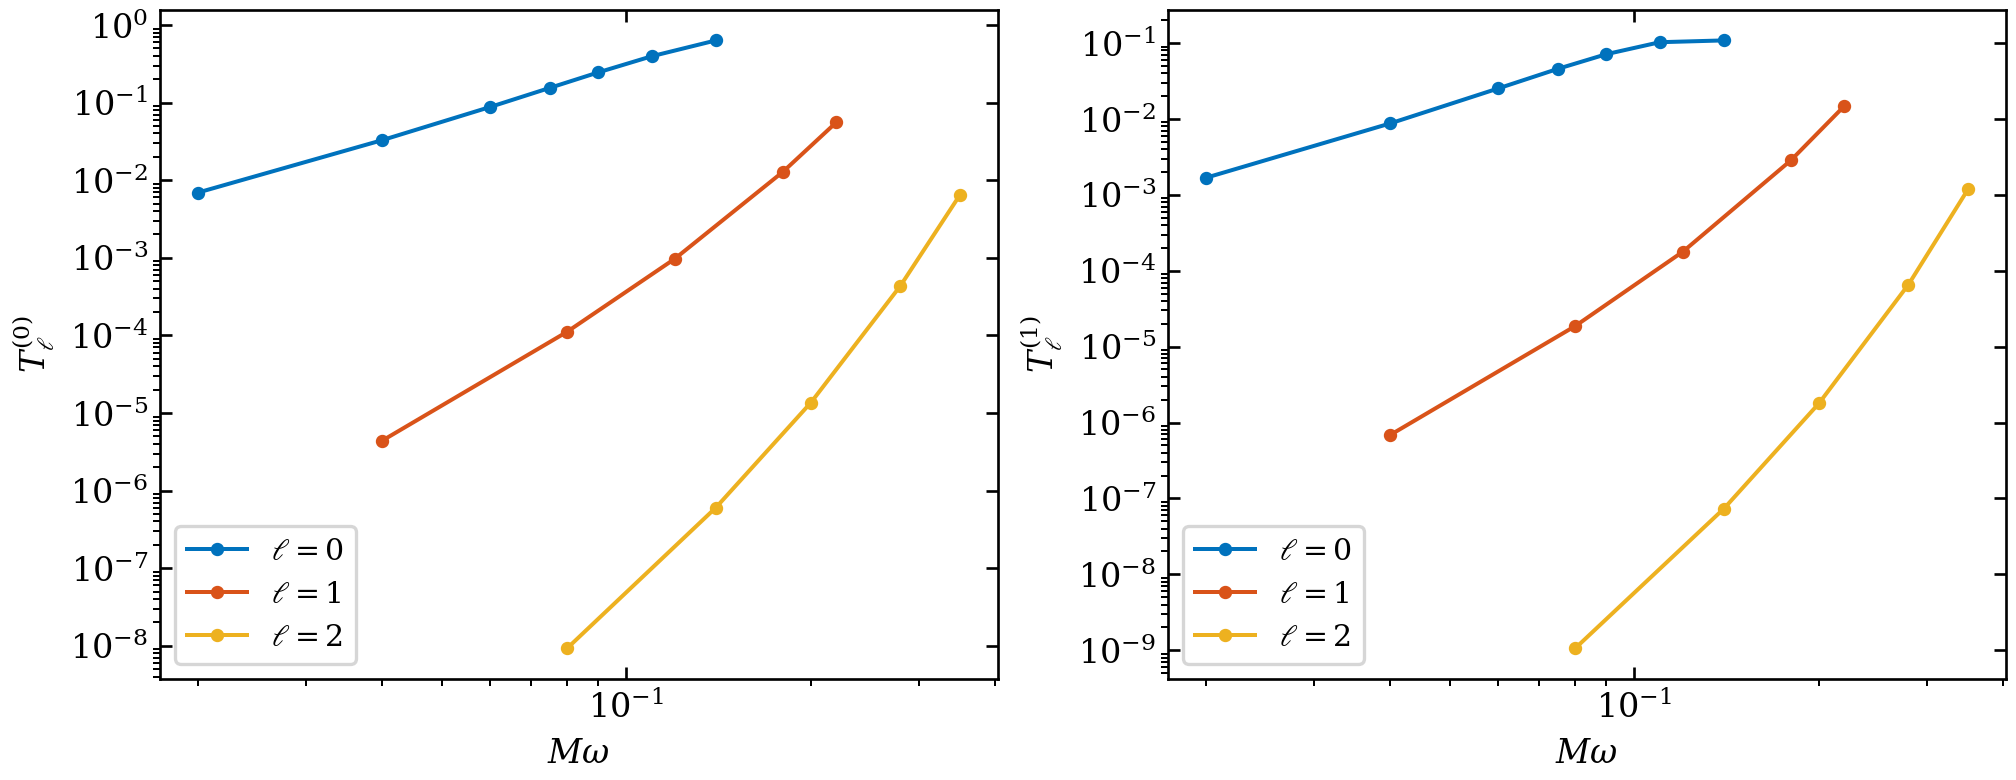
\includegraphics[width=0.92\textwidth]{../../figures/kerr_scalar_low_frequency_axisymmetric.png}
\caption{Low-frequency Kerr diagnostics for $a=0.5$, $m=0$, and
$\ell=0,1,2$.  Left: linear transmission coefficients.  Right:
self-channel nonlinear transmission coefficients.  The fitted low-frequency
slopes show that the Kerr fixed-incident coefficients decrease with the same
centrifugal hierarchy in $T^{(0)}$ and $T^{(1)}$.}
\label{fig:lowfreq}
\end{figure*}

\subsubsection{High-frequency behavior}

At high frequencies the phase-peeled homogeneous amplitudes become slowly
varying, while the nonlinear Green integral is controlled by rapidly
oscillatory tails.  The Schwarzschild calculation finds an exponential tail
with a fitted temperature close to the Hawking temperature~\cite{Hawking1975}.
For Kerr we do not assume the Schwarzschild asymptotic integral unchanged,
because the Teukolsky radial normalization and the $\Sigma$-weighted source
modify the integrand.  Instead we test the same one-parameter tail model,
\begin{equation}
T_\ell^{(1)}(\omega)\simeq
A_\ell\exp\left[-\frac{\omega}{T_{\rm fit}}\right],
\qquad
\omega>\operatorname{Re}\omega_{\ell0}.
\label{eq:boltzmann}
\end{equation}
For Kerr
\begin{equation}
T_H=\frac{\rp-\rmn}{4\pi(\rp^2+a^2)}.
\end{equation}
For $a=0.5$ the fits in Sec.~\ref{sec:results} give
$\pi M T_{\rm fit}=0.112$, $0.104$, and $0.100$ for
$\ell=0,1,2$, close to $\pi M T_H=0.1160$.  These values should be read as
finite-window effective temperatures rather than as a proof of an exact
high-frequency theorem.

\section{Results}
\label{sec:results}

Our main result on the Kerr nonlinear scattering coefficient is shown in
Fig.~\ref{fig:mainresults}.  This figure is the direct Kerr analogue of the
main Schwarzschild figure: it plots $T_\ell^{(1)}$ for $\ell=0,1,2$, uses a
linear scale to display the resonance peaks, and uses a logarithmic scale to
display the high-frequency tail.  The dashed lines mark the real parts of the
fundamental scalar Kerr quasinormal modes computed with the local
\texttt{qnm} package~\cite{Stein2019} for $s=0$, $a=0.5$, $m=0$, and $n=0$.

Three features are robust in the accepted data.  First, in the axisymmetric
Kerr cases studied here, $T_\ell^{(1)}$ is positive at every accepted sampled
frequency in the present flux
convention.  For positive coupling in Eq.~\eqref{eq:nonlinear_equation}, the
nonlinear correction therefore increases the absorbed flux and, by
Eq.~\eqref{eq:first_order_balance}, decreases the reflected flux at the same
order.  This sign statement refers to the coefficient convention of
Eqs.~\eqref{eq:T1} and \eqref{eq:R1}; it should not be compared to a reduced
Schwarzschild field convention without translating the flux normalization.

Second, the peaks of $T_\ell^{(1)}$ track the frequency scale set by the real
parts of the corresponding fundamental Kerr scalar QNMs~\cite{Berti2009,Stein2019}.  The fitted peak
positions are $M\omega_{\rm peak}=0.1299$, $0.3100$, and $0.5022$ for
$\ell=0,1,2$, while the QNM real parts are $0.1124$, $0.2979$, and $0.4920$.
The corresponding fractional offsets are approximately $16\%$, $4.1\%$, and
$2.1\%$.
To make the comparison quantitative without identifying the flux with a pole,
we fit the selected samples to the four-parameter profile
\begin{equation}
T_\ell^{(1)}(\omega)=T_{\rm off}+
\frac{A\,\gamma^2}{(M\omega-\omega_p)^2+\gamma^2} .
\label{eq:lorentzian}
\end{equation}
Here $\omega_p$ is the fitted center in units $M=1$, and $\gamma$ is the
half-width parameter of the interpolation.  This is the Kerr version of the
Breit-Wigner-type resonance observed in the Schwarzschild nonlinear
coefficients, not a claim that the flux itself is a meromorphic response.
The coefficient of determination of the three fits is $R^2=0.9974$,
$0.9979$, and $0.9991$ for $\ell=0,1,2$, respectively.  The comparison is
qualitative rather than a precision QNM determination: the nonlinear
coefficient is a real-frequency flux observable, whereas the QNM frequencies
are poles of the analytically continued response.
The quoted $\omega_{\rm peak}$ and $\gamma$ are parameters of the numerical
Lorentzian interpolation used to locate a broad feature; they are not a
claim that the nonlinear flux has been analytically continued to a QNM pole.
The fit uses the sampled points satisfying $T_\ell^{(1)}>0.2T_{\ell,\max}^{(1)}$;
the relative RMS residuals of these peak fits over the selected points are
$1.36\%$, $1.23\%$, and $0.57\%$ for $\ell=0,1,2$, respectively.  These
residuals quantify the descriptive quality of the interpolation, not an error
bar on the QNM frequencies.

Third, at high frequency the accepted tail points are well fit by the
Boltzmann form Eq.~\eqref{eq:boltzmann}.  The fitted temperatures differ from
the Kerr Hawking temperature by $3.2\%$, $10.1\%$, and $13.6\%$ for
$\ell=0,1,2$, respectively.  These are effective finite-window fit
parameters, not an analytic derivation of a thermal spectrum.  At low
frequency the Kerr fixed-incident coefficients decrease
with frequency in the accessible window.  This differs from simply copying the
Schwarzschild reduced-field statement and is therefore reported as a Kerr
numerical result rather than assumed analytically.

\begin{figure*}[t]
\centering
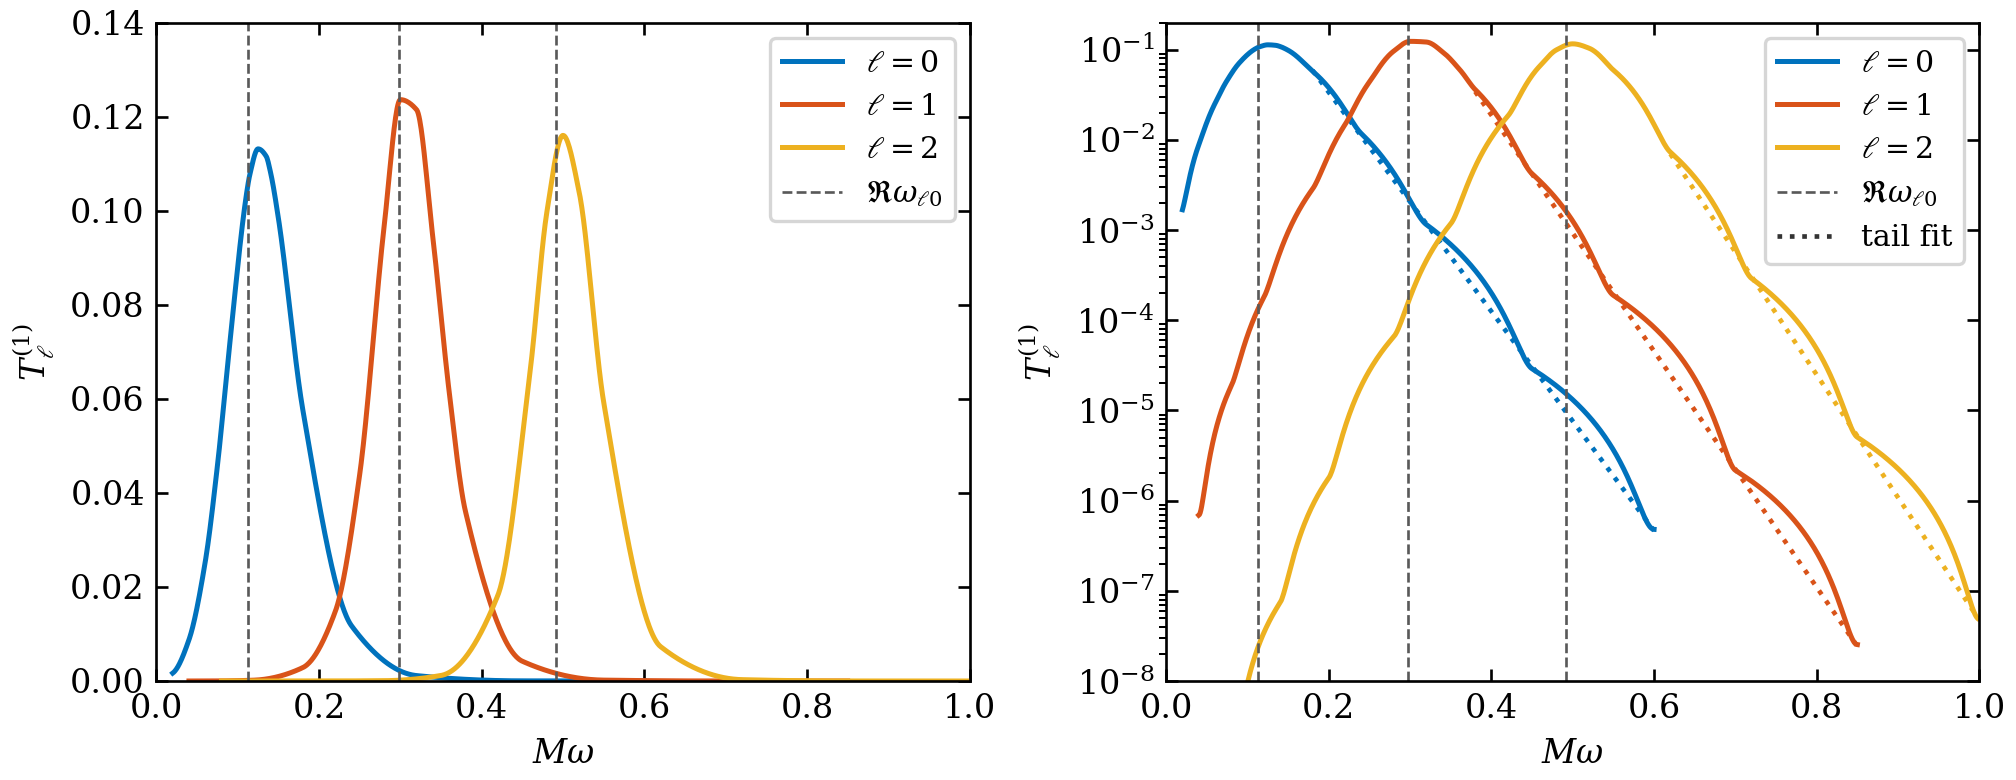
\includegraphics[width=0.92\textwidth]{../../figures/kerr_scalar_nonlinear_axisymmetric_fig2.png}
\caption{Nonlinear Kerr transmission coefficients
$T_\ell^{(1)}$ for $a=0.5$, $m=0$, and $\ell=0,1,2$.  The left panel uses a
linear scale to show the Breit-Wigner-type peaks.  The right panel uses a
logarithmic scale to show the exponential high-frequency tails; dotted
segments show the finite-window fits used in Table~\ref{tab:fit}.  Dashed
vertical lines mark the real parts of the fundamental scalar Kerr QNMs
$\operatorname{Re}\omega_{\ell0}$.}
\label{fig:mainresults}
\end{figure*}

\begin{table}[t]
\caption{Fitting parameters of the Kerr nonlinear transmission resonance and
the high-frequency Boltzmann tail.  The QNM frequencies are scalar Kerr
fundamental modes with $s=0$, $a=0.5$, $m=0$, and $n=0$.  All frequencies are
reported in units $M=1$.}
\label{tab:fit}
\begin{ruledtabular}
\begin{tabular}{c c c c c c c}
$\ell$ & $\omega_p$ & $\gamma$
& $\Re\omega_Q$
& $|\Im\omega_Q|$
& $\pi T_{\rm fit}$
& $\Delta T$\\
\hline
0 & 0.1299 & 0.0779 & 0.1124 & 0.1022 & 0.1123 & 3.25\%\\
1 & 0.3100 & 0.0597 & 0.2979 & 0.0954 & 0.1043 & 10.1\%\\
2 & 0.5022 & 0.0611 & 0.4920 & 0.0946 & 0.1003 & 13.6\%\\
\end{tabular}
\end{ruledtabular}
\end{table}

The exponential fits use unweighted least squares for
$\log T_\ell^{(1)}$ versus $M\omega$ over the windows
$[0.18,0.60]$, $[0.38,0.85]$, and $[0.62,1.00]$ for
$\ell=0,1,2$, respectively.  The corresponding root-mean-square residuals
in log space are $4.5\times10^{-2}$, $4.9\times10^{-2}$, and
$3.8\times10^{-2}$.  These window-dependent residuals quantify the quality
of the finite-window fit; they are not estimates of a systematic error outside
the computed frequency range.

Because the effective temperature is a fit diagnostic rather than an analytic
observable, we also repeat the tail fit after shifting either edge of each
window while retaining at least three positive data points.  The resulting
window ranges and the largest logarithmic fit residual are given in
Table~\ref{tab:tail-window}.  The fitted values vary only at the percent level
within these local windows, while their absolute offsets from $T_H$ remain
consistent with the finite-window qualification above.

\begin{table*}[t]
\caption{Sensitivity of the finite-window effective temperatures to the fit
window.  The baseline window is the one used in Table~\ref{tab:fit}; the range
is obtained from three nearby edge-shifted windows.  The final column is the
largest absolute fractional offset from the Kerr Hawking temperature among
the four windows.}
\label{tab:tail-window}
\begin{ruledtabular}
\begin{tabular}{c c c c c c}
$\ell$ & baseline $[M\omega_{\min},M\omega_{\max}]$
& $\pi T_{\rm fit}^{\rm base}$ & range of $\pi T_{\rm fit}$
& $\max\sigma_{\log}$ & $\max|T_{\rm fit}/T_H-1|$\\
\hline
0 & $[0.18,0.60]$ & 0.1123 & $[0.1112,0.1131]$ & $4.83\times10^{-2}$ & 4.18\%\\
1 & $[0.38,0.85]$ & 0.1043 & $[0.1034,0.1057]$ & $4.87\times10^{-2}$ & 10.90\%\\
2 & $[0.62,1.00]$ & 0.1003 & $[0.0994,0.1012]$ & $3.82\times10^{-2}$ & 14.37\%\\
\end{tabular}
\end{ruledtabular}
\end{table*}

For the accepted subset of the sweep, the largest first-order balance residual
is $4.3\times10^{-12}$, $2.2\times10^{-12}$, and
$1.2\times10^{-12}$ for $\ell=0,1,2$, respectively.  The full sweep also
contains rejected lowest-frequency points with residuals as large as
$3.9\times10^{-5}$ and $1.2\times10^{-4}$ for $\ell=1,2$; these are caused by
cancellation in the reflected interference term and are not used for precision
claims.  The transmitted coefficients remain smooth at those frequencies, so
we retain them for the low-frequency slope measurement but explicitly separate
that trend from an accuracy claim for $R^{(1)}$.

\begin{table*}[t]
\caption{Numerical quality of the axisymmetric Kerr frequency sweeps.  Here
$\delta_0=|T^{(0)}+R^{(0)}-1|$ and
$\delta_1=|T^{(1)}+R^{(1)}|$.  A point is counted as accepted when
$\delta_1\le 10^{-8}$.  All active frequency-sweep points use the refined
resolution $N=240$ and quadrature order $q=192$; the earlier $N=224$, $q=160$
sweep is retained only as the production-resolution audit in
Table~\ref{tab:production-convergence}.  The final column is the
root-mean-square residual of the logarithmic high-frequency tail fit.}
\label{tab:numerics}
\begin{ruledtabular}
\begin{tabular}{c c c c c c}
$\ell$ & points & $\max\delta_0$ & accepted & $\max\delta_1^{\rm acc}$
& $\sigma_{\rm tail}$\\
\hline
0 & 16 & $2.2\times10^{-11}$ & 16/16 & $4.3\times10^{-12}$ & $4.5\times10^{-2}$\\
1 & 16 & $1.9\times10^{-11}$ & 14/16 & $2.2\times10^{-12}$ & $4.9\times10^{-2}$\\
2 & 15 & $3.8\times10^{-11}$  & 12/15 & $1.2\times10^{-12}$ & $3.8\times10^{-2}$\\
\end{tabular}
\end{ruledtabular}
\end{table*}

The change from the former production resolution to the active refined
resolution is quantified separately in Table~\ref{tab:production-convergence}.
At the representative peak points the refined calculation changes the
transmission coefficient by at most $3.2\times10^{-5}$ and preserves the
first-order flux balance at the $10^{-12}$ level.  We therefore use the
refined curves for the physical discussion below; the lower-resolution values
are reported to make the resolution choice auditable rather than folded into
an unreported systematic error.

\begin{table*}[t]
\caption{Production-resolution audit for the axisymmetric Kerr calculation.
The entries compare the former production configuration $(N,q)=(224,160)$
with the active reference configuration $(N,q)=(240,192)$ at fixed
$r_{\rm m}=40$.  Each entry in the first four columns is
$|X_{240,192}-X_{224,160}|/|X_{240,192}|$ for the indicated Green-function
amplitude or flux coefficient; the final column is the
absolute first-order balance residual of the reference run.}
\label{tab:production-convergence}
\begin{ruledtabular}
\begin{tabular}{c c c c c c}
case & $\Delta A_{\rm ref}$ & $\Delta A_H$
& $\Delta T^{(1)}$ & $\Delta R^{(1)}$ & $|\delta_1|_{\rm ref}$\\
\hline
$\ell=0,\ M\omega=.125$ & $4.5\times10^{-7}$ & $7.8\times10^{-7}$
& $2.3\times10^{-6}$ & $2.3\times10^{-6}$ & $2.7\times10^{-12}$\\
$\ell=1,\ M\omega=.34$ & $5.9\times10^{-6}$ & $3.3\times10^{-6}$
& $1.5\times10^{-5}$ & $1.5\times10^{-5}$ & $2.2\times10^{-12}$\\
$\ell=2,\ M\omega=.52$ & $9.6\times10^{-6}$ & $7.6\times10^{-6}$
& $3.1\times10^{-5}$ & $3.1\times10^{-5}$ & $1.2\times10^{-12}$\\
\end{tabular}
\end{ruledtabular}
\end{table*}

We additionally test the self channel with $\ell=m=2$ at both signs of the
Kerr horizon frequency $p$ and for a rapidly rotating case.  Table~\ref{tab:convergence}
records finite-resolution changes under $N$, $r_{\rm m}$, and $q$; these are
not rigorous error bounds.  The horizon amplitude is less sensitive than the
reflected amplitude, while the Wronskian error remains below
$6\times10^{-16}$.  We therefore use flux balance, rather than one amplitude
difference, as the acceptance criterion.

\begin{table*}[t]
\caption{Method-level convergence stress tests for the scalar Kerr Green
integrals.  Each entry is the maximum relative change in the indicated
amplitude over the non-reference runs.  The $N$ scan compares $N=224,288$ with
$N=256$; the matching scan compares the listed alternatives with the reference
$r_{\rm m}$; and the quadrature scan compares lower orders with $q=192$.
These non-axisymmetric self-channel tests are validation data for the numerical
method and are not included in the axisymmetric production curves.}
\label{tab:convergence}
\begin{ruledtabular}
\begin{tabular}{c c c c c c c c}
case & $\Delta A_{\rm ref}[N]$ & $\Delta A_H[N]$
& $\Delta A_{\rm ref}[r_{\rm m}]$ & $\Delta A_H[r_{\rm m}]$
& $\Delta A_{\rm ref}[q]$ & $\Delta A_H[q]$ & $\max\delta_W$\\
\hline
$a=.5,\ M\omega=.24$ & $2.1\times10^{-5}$ & $1.1\times10^{-7}$
& $3.3\times10^{-5}$ & $5.4\times10^{-8}$ & $2.8\times10^{-8}$
& $2.5\times10^{-8}$ & $5.9\times10^{-16}$\\
$a=.5,\ M\omega=.30$ & $3.8\times10^{-5}$ & $2.8\times10^{-8}$
& $2.0\times10^{-5}$ & $4.4\times10^{-8}$ & $1.8\times10^{-6}$
& $1.7\times10^{-6}$ & $3.7\times10^{-16}$\\
$a=.9,\ M\omega=.58$ & $1.5\times10^{-6}$ & $1.2\times10^{-8}$
& $1.7\times10^{-6}$ & $9.4\times10^{-9}$ & $1.4\times10^{-10}$
& $5.1\times10^{-7}$ & $2.9\times10^{-16}$\\
\end{tabular}
\end{ruledtabular}
\end{table*}

\noindent\parbox[t]{0.96\columnwidth}{\small
\textit{Local field diagnostic.}\\
At the representative peak in Fig.~\ref{fig:accuracy}, the field-dependent
radial residual has maximum, 95th-percentile, and median values
$2.5\times10^{-10}$, $3.3\times10^{-12}$, and $1.3\times10^{-13}$.\\
The largest normalized Chebyshev tail is $2.8\times10^{-14}$ and the
Wronskian mismatch is below $3\times10^{-16}$.  These local diagnostics are
reported separately from the global flux-balance residual.}

\begin{figure*}[t]
\centering
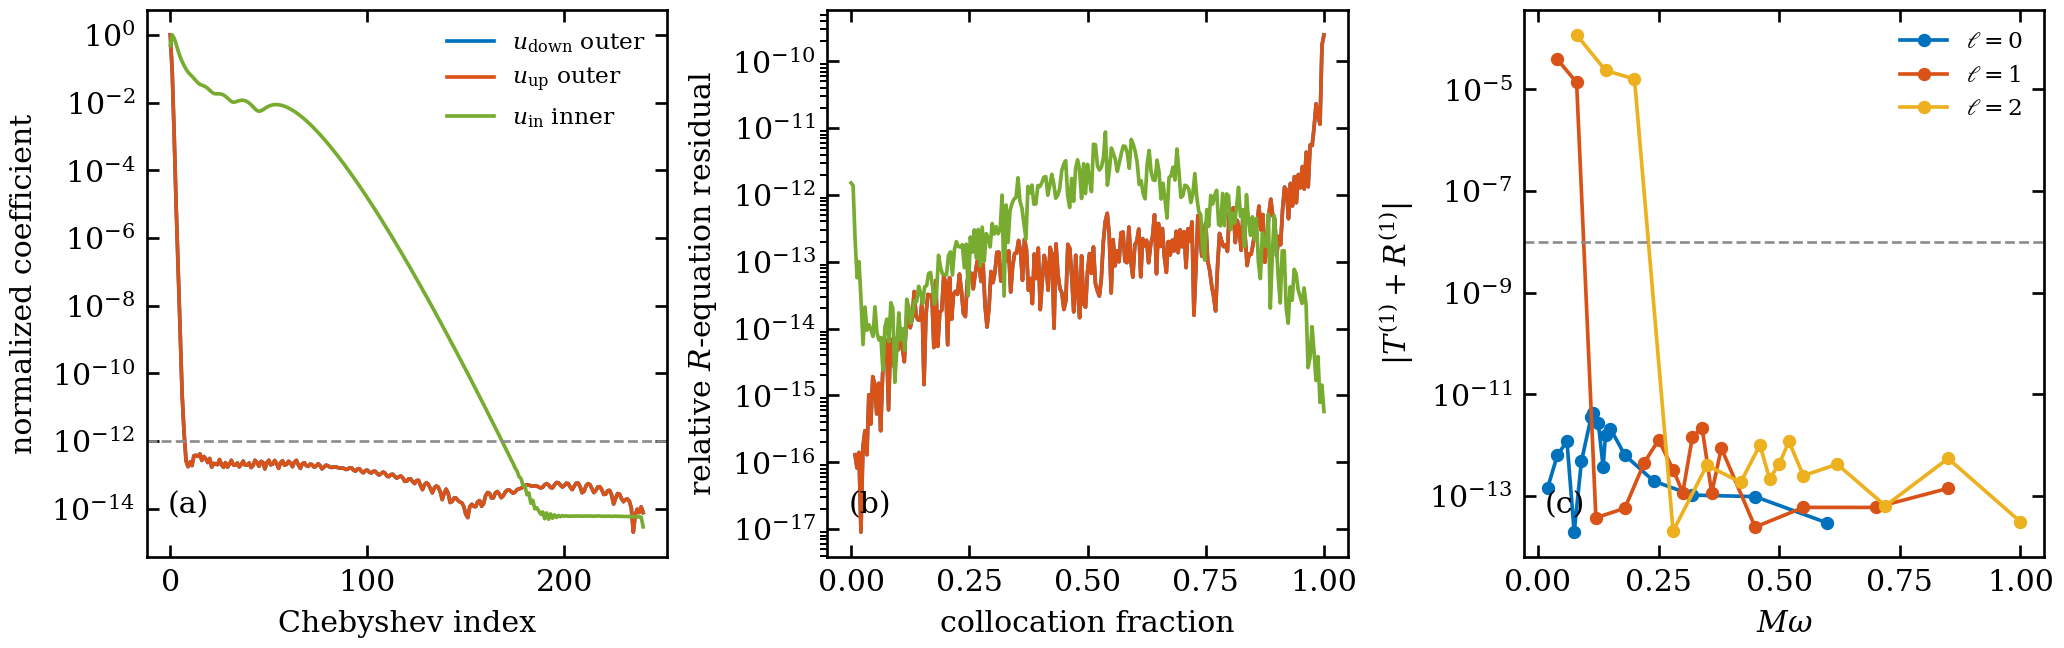
\includegraphics[width=0.95\textwidth]{../../figures/kerr_scalar_axisymmetric_accuracy.png}
\caption{Internal numerical accuracy diagnostics for the axisymmetric Kerr
calculation.  Panels (a) and (b) use the representative peak point
$a=0.5$, $m=0$, $\ell=2$, and $M\omega=0.52$ with $N=240$ and quadrature order
$q=192$.  Panel (a) shows the normalized Chebyshev coefficients of the
phase-peeled homogeneous solutions on the outer and inner subdomains.  Panel
(b) shows the relative residual \eqref{eq:radial_residual} after substituting
the numerical solution back into the original radial Teukolsky equation.
Panel (c) shows the first-order flux-balance residual over the full
axisymmetric frequency sweep.  The dashed line marks the acceptance threshold
$10^{-8}$ used in Table~\ref{tab:numerics}.}
\label{fig:accuracy}
\end{figure*}

\subsection{Target-channel structure}

The spheroidal source projection is a genuinely Kerr-specific part of the
calculation.  To expose it directly, we evaluated the target channels
$\ell'=2,\ldots,6$ for the representative mode
$(a,\ell,m,M\omega)=(0.5,2,2,0.30)$ using $N=288$, quadrature order
$q=224$, and Fourier-tail tolerance $10^{-11}$.  The amplitudes in
Table~\ref{tab:channels} use the unit-horizon normalization of
Eq.~\eqref{eq:bc_hor}; they are not fixed-incident flux coefficients.
Odd target channels vanish by the even-parity angular projectors in
Eq.~\eqref{eq:source}, while the even channels span several orders of
magnitude in the outgoing Green amplitude.

\begin{table*}[t]
\caption{Representative Kerr target-channel matrix for an incident
$(a,\ell,m,M\omega)=(0.5,2,2,0.30)$ mode.  The angular entries are absolute
values of the two source projectors in Eq.~\eqref{eq:source}; the Green
amplitudes are unit-horizon first-order amplitudes.  The odd channels vanish
within the displayed precision.}
\label{tab:channels}
\begin{ruledtabular}
\begin{tabular}{c c c c c}
$\ell'$ & $|C^{(0)}_{\ell'\ell m}|$ & $|C^{(2)}_{\ell'\ell m}|$
& $|A_{{\rm ref},\ell'|\ell m}^{(1)}|$
& $|A_{H,\ell'|\ell m}^{(1)}|$\\
\hline
2 & $1.136\times10^{-1}$ & $1.034\times10^{-2}$ & $1.137\times10^{6}$ & $3.804\times10^{3}$\\
3 & $0$ & $0$ & $0$ & $0$\\
4 & $3.578\times10^{-2}$ & $5.513\times10^{-3}$ & $1.362\times10^{4}$ & $1.319$\\
5 & $0$ & $0$ & $0$ & $0$\\
6 & $5.341\times10^{-3}$ & $5.364\times10^{-3}$ & $2.265\times10^{3}$ & $5.383\times10^{-7}$\\
\end{tabular}
\end{ruledtabular}
\end{table*}

The channel scan is converged for the dominant reflected amplitudes: changing
$N$ from 256 to 288 changes $A_{\rm ref}^{(1)}$ by
$2.5\times10^{-7}$ in the self channel and by $6.3\times10^{-7}$ in the
$\ell'=4$ channel.  The corresponding $\ell'=4$ horizon amplitude changes by
$7.1\times10^{-3}$, whereas the $\ell'=6$ horizon amplitude is close to the
double-precision cancellation floor and changes by order unity.  For the
displayed $\ell'=6$ row, the independent diagnostic
$(|B_{\rm inc}|^2+|B_{\rm ref}|^2)/||B_{\rm inc}|^2-|B_{\rm ref}|^2|$
is $3.27\times10^{13}$; this is the relevant conditioning indicator for the
horizon-normalized continuation.  We therefore use this experiment to
establish the target-channel structure and the dominant outgoing amplitudes,
not to claim uniform high precision for every off-diagonal horizon coefficient.
Since off-diagonal channels do not
interfere with the zeroth-order field, their energy flux first enters at
$\mathcal O(\epsilon^2)$.

\subsection{Non-axisymmetric superradiant check}

The axisymmetric production sweep is useful for a controlled comparison with
the Schwarzschild calculation, but it removes the most distinctive rotating
black-hole effect because $p=\omega$ when $m=0$.  We therefore performed a
bounded check with $a=0.5$ and $\ell=m=2$, using $N=320$ on both spectral
subdomains, quadrature order $q=320$, and $r_{\rm m}=40M$.  The threshold is
$m\Omega_H=0.2679491924$.  The full ten-point scan is retained in the tracked
CSV file; Table~\ref{tab:superradiant} lists only points satisfying the same
first-order balance gate $|T^{(1)}+R^{(1)}|\leq10^{-8}$ used for the production
data.  The rejected points are $M\omega=0.20,0.22,0.255,0.265,0.28$; they lie
in the near-threshold portion of the scan and are limited by cancellation in
the reflected interference term, rather than by a physical discontinuity.

Figure~\ref{fig:superradiant} shows the signed linear and first-order horizon
flux coefficients.  On the accepted points below the threshold, both
$T^{(0)}$ and $T^{(1)}$ are negative, while they are positive on the accepted
points above it.  Thus the scalar Kerr calculation recovers the expected
signed-flux change across the superradiant boundary in this representative
mode.  This is a validation of the horizon-frequency normalization, not a
systematic survey over spin, $m$, or spheroidal target channels.

\begin{figure*}[t]
\centering
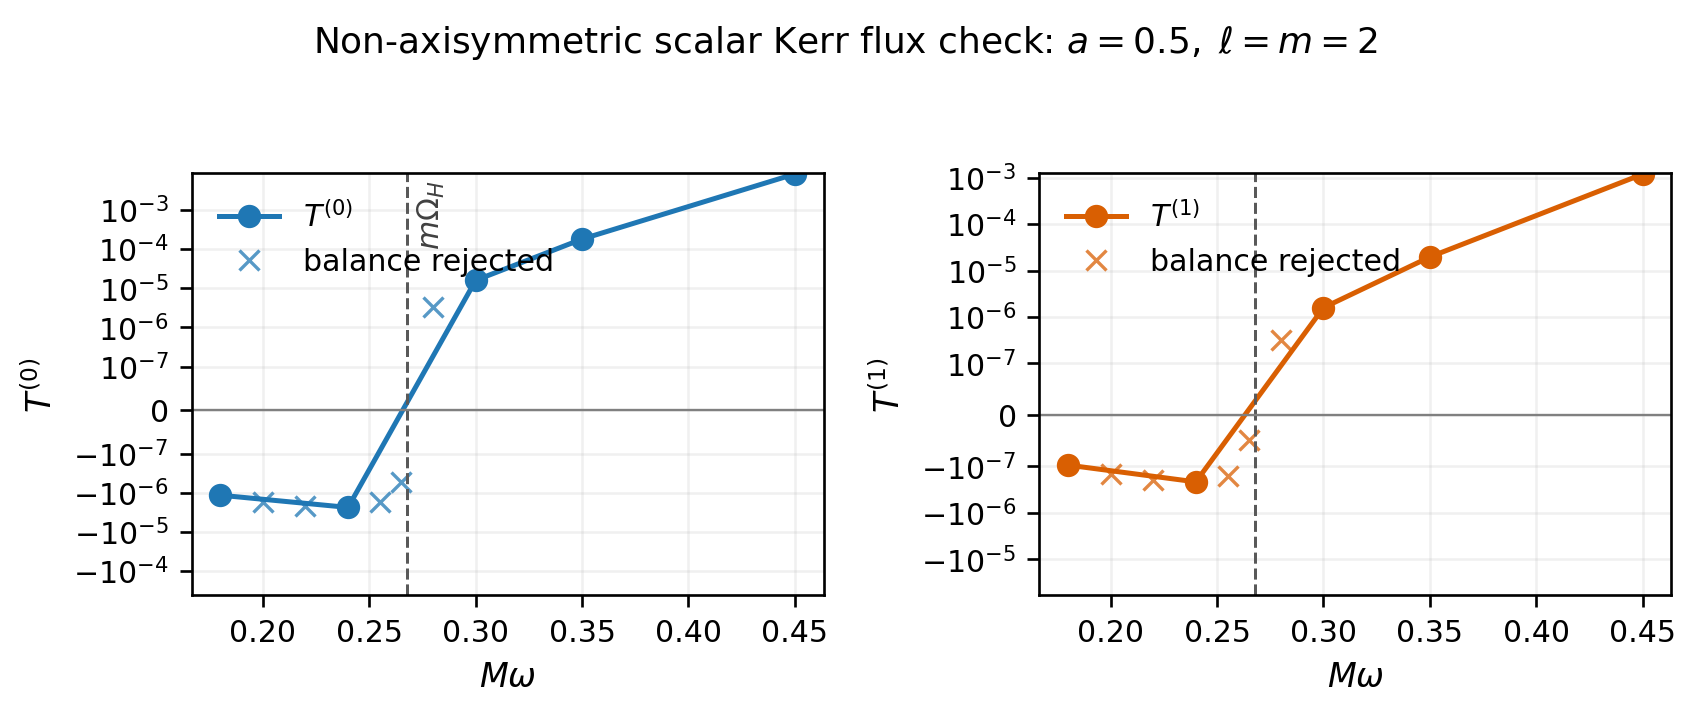
\includegraphics[width=0.88\textwidth]{../../figures/kerr_scalar_nonlinear_superradiant_m2.png}
\caption{Bounded non-axisymmetric scalar Kerr flux check for $a=0.5$ and
$\ell=m=2$.  The dashed line marks $M\omega=m\Omega_H=0.2679491924$.
Filled circles satisfy the first-order balance gate; crosses mark scan points
retained in the CSV file but rejected because of cancellation.  The signed
coefficients change sign across the superradiant threshold on the accepted
points.}
\label{fig:superradiant}
\end{figure*}

\begin{table*}[t]
\caption{Accepted points in the bounded non-axisymmetric superradiant check.
The entries are signed energy-flux coefficients for $a=0.5$ and $\ell=m=2$;
$p=\omega-m\Omega_H$.  The omitted points in the ten-point scan fail the
$10^{-8}$ first-order balance gate.}
\label{tab:superradiant}
\begin{ruledtabular}
\begin{tabular}{c c c c c}
$M\omega$ & $p$ & $T^{(0)}$ & $T^{(1)}$ & $|T^{(1)}+R^{(1)}|$\\
\hline
0.18 & $-8.795\times10^{-2}$ & $-1.157\times10^{-6}$ & $-9.742\times10^{-8}$ & $4.788\times10^{-13}$\\
0.24 & $-2.795\times10^{-2}$ & $-2.373\times10^{-6}$ & $-2.153\times10^{-7}$ & $1.261\times10^{-12}$\\
0.30 & $3.205\times10^{-2}$ & $1.595\times10^{-5}$ & $1.582\times10^{-6}$ & $9.240\times10^{-13}$\\
0.35 & $8.205\times10^{-2}$ & $1.804\times10^{-4}$ & $1.960\times10^{-5}$ & $1.598\times10^{-12}$\\
0.45 & $1.821\times10^{-1}$ & $8.298\times10^{-3}$ & $1.194\times10^{-3}$ & $4.130\times10^{-12}$\\
\end{tabular}
\end{ruledtabular}
\end{table*}

\subsection{Kerr-to-Schwarzschild continuity}

As a limiting-case check independent of external reference calculations, we
hold $(\ell,m,M\omega)=(2,0,0.52)$ fixed and sweep the dimensionless spin from
$a/M=0$ to $0.5$.  The scalar spheroidal eigenvalue, the covariant source
projection, the scattering amplitudes, and both flux coefficients are
recomputed at every spin.  At $a=0$ the angular basis becomes spherical and the
endpoint formulation reduces to the Schwarzschild spectral route; no radial
endpoint is removed or replaced by a finite horizon cutoff.  Figure~\ref{fig:spin-limit}
shows that $T^{(1)}$ and $-R^{(1)}$ vary smoothly from the $a=0$ value, while
Table~\ref{tab:spin-limit} records the balance and Wronskian diagnostics for
the same points.  The largest absolute first-order balance residual in this
scan is $1.4\times10^{-12}$ and the largest linear balance residual is below
$1.2\times10^{-11}$.  This experiment is a continuity and implementation
check; it is not used as an external reference result or as a claim that the Kerr and
Schwarzschild coefficient conventions are identical without the conversion in
Appendix~\ref{app:flux}.

\begin{figure*}[t]
\centering
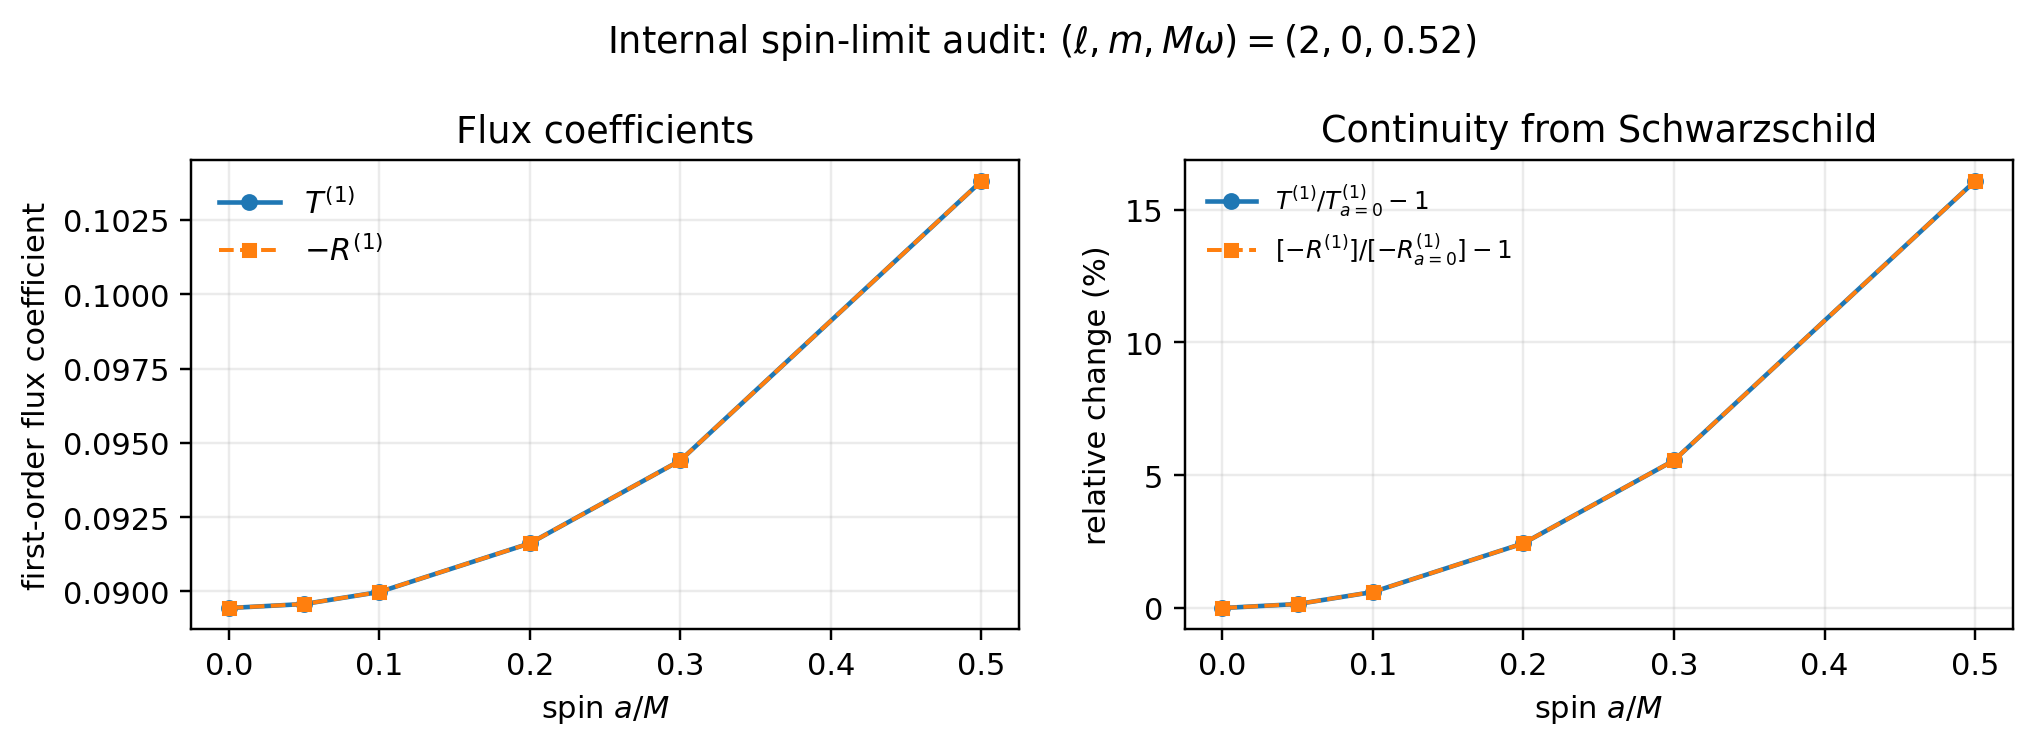
\includegraphics[width=0.92\textwidth]{../../figures/kerr_scalar_spin_limit.png}
\caption{Internal Kerr-to-Schwarzschild continuity test at fixed
$(\ell,m,M\omega)=(2,0,0.52)$.  The first-order transmission coefficient and
$-R^{(1)}$ remain paired by the flux balance while changing smoothly with
$a/M$.  The right panel normalizes both coefficients to the $a=0$ value; all
points use the endpoint-inclusive spectral solver and are accepted by the
first-order balance check.}
\label{fig:spin-limit}
\end{figure*}

\begin{table*}[t]
\caption{Internal Kerr-to-Schwarzschild spin-limit audit for
$(\ell,m,M\omega)=(2,0,0.52)$.  The entries use the same fixed-incident
normalization as the production coefficients.  The two balance columns are
$T^{(0)}+R^{(0)}-1$ and $T^{(1)}+R^{(1)}$, respectively.}
\label{tab:spin-limit}
\begin{ruledtabular}
\begin{tabular}{c c c c c c}
$a/M$ & $T^{(1)}$ & $R^{(1)}$ & $|\delta_0|$ & $|\delta_1|$ & $|\delta_W|$\\
\hline
0.00 & $8.94395\times10^{-2}$ & $-8.94395\times10^{-2}$ & $1.1\times10^{-12}$ & $3.8\times10^{-13}$ & $2.6\times10^{-16}$\\
0.05 & $8.95742\times10^{-2}$ & $-8.95742\times10^{-2}$ & $9.8\times10^{-12}$ & $1.1\times10^{-12}$ & $3.3\times10^{-16}$\\
0.10 & $8.99794\times10^{-2}$ & $-8.99794\times10^{-2}$ & $3.7\times10^{-12}$ & $4.9\times10^{-13}$ & $0$\\
0.20 & $9.16178\times10^{-2}$ & $-9.16178\times10^{-2}$ & $4.3\times10^{-13}$ & $7.6\times10^{-14}$ & $1.8\times10^{-16}$\\
0.30 & $9.44095\times10^{-2}$ & $-9.44095\times10^{-2}$ & $1.1\times10^{-11}$ & $1.3\times10^{-12}$ & $1.8\times10^{-16}$\\
0.50 & $1.03814\times10^{-1}$ & $-1.03814\times10^{-1}$ & $6.0\times10^{-12}$ & $1.2\times10^{-12}$ & $0$\\
\end{tabular}
\end{ruledtabular}
\end{table*}

\section{Discussion and outlook}

We have formulated the weakly nonlinear scattering problem for a scalar field
on Kerr in a way that keeps the observable content of the Schwarzschild
Green-function calculation unchanged.  The linear in solution is normalized at
the horizon, the incident normalization is restored through $\Bin$, and the
nonlinear corrections are read from the interference terms in the physical
energy fluxes.  In this form the two useful balance laws,
$T^{(0)}+R^{(0)}=1$ and $T^{(1)}+R^{(1)}=0$, remain the main global checks of
the calculation.  The extension is not a formal replacement of the
Schwarzschild radial variable by a Kerr one: the horizon frequency
$p=\omega-m\Omega_H$, spheroidal angular basis, and $\Sigma$-weighted nonlinear
source all enter the normalization of the observable coefficients.

For the axisymmetric Kerr sample $a=0.5$, $m=0$, and $\ell=0,1,2$, the present
numerical diagnostics support the following qualitative picture.  The nonlinear
transmission coefficient develops a single dominant Breit-Wigner-type peak for
each $\ell$, with the peak position tracking the frequency scale of the corresponding
scalar Kerr quasinormal mode.  The high-frequency tail is well fit by an
exponential form in the computed window, and the fitted temperature is of the
same order as the Kerr Hawking temperature.  At low frequency, however, the
fixed-incident Teukolsky normalization and the Kerr source weight prevent a
direct transcription of the Schwarzschild reduced-variable scaling; the
low-frequency behavior is therefore treated here as a numerical Kerr result.

The present data also identify the current limiting numerical effect.  The
transmitted nonlinear coefficient is smooth across the displayed low-frequency
windows, while the reflected coefficient can suffer large cancellations in the
interference integral.  This is why the lowest-frequency $\ell=1,2$ points are
used for the scaling trend but are not counted as high-precision reflected-flux
points in Table~\ref{tab:numerics}.  The numerical evidence is therefore
strongest for the resonance region, the high-frequency tail, and the
transmitted low-frequency scaling; it is weaker for the individual
low-frequency reflected coefficient before using the balance law.  The
representative target-channel experiment in Table~\ref{tab:channels}
demonstrates the matrix structure generated by the Kerr source projection and
shows that the dominant reflected off-diagonal amplitudes can be resolved at
the stated spectral order.  A broader scan over $(a,\ell,m,\omega)$, uniform
acceptance gates for off-diagonal horizon amplitudes, and a systematic study of
the superradiant nonlinear flux remain future work.

The spin-limit audit supplies an additional implementation-level check.  We
fix $(\ell,m)=(2,0)$ and $M\omega=0.52$; the first-order coefficients change
smoothly from the $a=0$ endpoint to the production value at $a=0.5$, while the
two flux-balance laws remain satisfied.  This continuity test does not replace a
convention-matched Schwarzschild comparison, but it rules out a discontinuity
introduced solely by the Kerr tortoise coordinate, spheroidal projection, or
endpoint matching.

\subsection{Scope and limitations}

The conclusions above have a deliberately narrow interpretation.  The
calculation is a fixed-background scalar response problem with a prescribed
cubic interaction; it is not a second-order metric perturbation, a
gravitational self-force calculation, or an EMRI waveform model.  The main
frequency sweep is axisymmetric.  The separate $m=2$ check tests one narrow
superradiant crossing but does not provide a systematic survey of superradiant
sign changes.  The target-channel experiment establishes the spheroidal
coupling structure and the dominant reflected amplitudes, but the
$\ell'=6$ horizon coefficient is conditioning limited in double precision.
The QNM comparison uses real-frequency peak locations only, and the
finite-window exponential fits should not be interpreted as QNM residues or
as a proof of Hawking thermality.  Extending the result to generic Kerr
orbits or to gravitational perturbations requires, respectively,
source-harmonic and orbit-evolution modules or metric reconstruction, gauge
completion, and regularization; none of these are hidden in the present
scalar result.

\section*{Data and code availability}

The numerical data used in Figs.~\ref{fig:lowfreq}--\ref{fig:spin-limit} and
Tables~\ref{tab:fit}, \ref{tab:numerics}, \ref{tab:production-convergence},
\ref{tab:convergence}, \ref{tab:channels}, \ref{tab:superradiant}, and
\ref{tab:spin-limit} are included in the project
data directory, ``results/''.  The figures are generated by the scripts in
``scripts/'', and the exact commands and tracked inputs are listed in
``docs/prd/README.md''.  The source code and frozen inputs are maintained at
\url{https://github.com/ljq2088/KerrScattering}.  The numerical checker compares the rounded entries in
Tables~\ref{tab:fit}--\ref{tab:channels}, the spin-limit audit, the
production-resolution audit, and the low-frequency slopes with the tracked CSV
files.  The artifact
manifest records file sizes and SHA-256 hashes for the figure and CSV inputs,
including the target-channel values in Table~\ref{tab:channels}; a human-readable
snapshot is provided in ``docs/prd/reproducibility\_report.md''.  No external
experimental data are used.

\appendix

\section{Flux normalizations}
\label{app:flux}

\subsection{Projected Kerr source}

The scalar wave equation separates only after multiplying by
$\Sigma=r^2+a^2\cos^2\theta$.  At first order this gives
\begin{equation}
\Sigma\Box\Phi^{(1)}=-\Sigma|\Phi^{(0)}|^2\Phi^{(0)} .
\end{equation}
Using
\begin{align}
\Phi^{(0)}
&=e^{-\ii\omega t+\ii m\phi}S_{\ell m}R_{\ell m\omega},
\nonumber\\
\Phi^{(1)}
&=e^{-\ii\omega t+\ii m\phi}
\sum_{\ell'}S_{\ell'm}R^{(1)}_{\ell'|\ell m\omega},
\end{align}
and projecting with $S_{\ell'm}^*$ gives
\begin{equation}
\mathcal L_{\ell'm\omega}R^{(1)}_{\ell'|\ell m\omega}
=-\left(r^2C^{(0)}_{\ell'\ell m}
+a^2C^{(2)}_{\ell'\ell m}\right)
|R_{\ell m\omega}^{\rm in}|^2R_{\ell m\omega}^{\rm in}.
\end{equation}
Here
\begin{equation}
C^{(j)}_{\ell'\ell m}=
\int \dd\Omega\,\cos^j\theta\,
S_{\ell'm}^*|S_{\ell m}|^2S_{\ell m},
\qquad j=0,2 .
\end{equation}
This is the point at which Kerr differs from the spherical Schwarzschild
reduction: a single incident spheroidal channel sources a matrix of target
channels with the same $m$.  Only the target channel $\ell'=\ell$ contributes
linearly to the total flux, because only that channel interferes with the
zeroth-order outgoing field.  Off-diagonal channels contribute to the energy
flux first at order $\epsilon^2$.

\subsection{Linear current}

The scalar radial current is
\begin{equation}
J[R]=\frac{\DeltaK}{2\ii}
\left(R^*\frac{\dd R}{\dd r}-R\frac{\dd R^*}{\dd r}\right).
\end{equation}
Using the asymptotics in Eq.~\eqref{eq:bc_inf}, the far-zone current is
\begin{equation}
J_\infty=-\omega|\Bin|^2+\omega|\Bref|^2 .
\end{equation}
At the horizon, Eq.~\eqref{eq:bc_hor} gives
\begin{equation}
J_H=-p(\rp^2+a^2).
\end{equation}
The equality $J_\infty=J_H$ gives
Eq.~\eqref{eq:linear_balance}.

\subsection{Fixed-incident nonlinear flux}

The Green-function amplitudes $\Aref$ and $\AH$ are computed with the
zeroth-order in solution normalized to unit horizon amplitude.  Scattering
coefficients, however, are defined at fixed incident amplitude.  Therefore we
rescale the zeroth-order solution by
\begin{equation}
\alpha=\frac{1}{\Bin}.
\end{equation}
Because the source is cubic, the first-order field scales as
$|\alpha|^2\alpha$.  The fixed-incident self-channel field has the asymptotic
form
\begin{align}
R_{\rm fix}\sim
\frac{e^{-\ii\omega r_*}}{r}
\nonumber\\
\quad
+\left(\frac{\Bref}{\Bin}
+\epsilon\frac{\Aref}{|\Bin|^2\Bin}\right)
\frac{e^{+\ii\omega r_*}}{r},
\qquad r\rightarrow\infty ,
\end{align}
and
\begin{equation}
R_{\rm fix}\sim
\left(\frac{1}{\Bin}
+\epsilon\frac{\AH}{|\Bin|^2\Bin}\right)
e^{-\ii p r_*},
\qquad r\rightarrow\rp .
\end{equation}
The transmitted flux coefficient is therefore
\begin{align}
T&=\frac{p(\rp^2+a^2)}{\omega}
\left|
\frac{1}{\Bin}
+\epsilon\frac{\AH}{|\Bin|^2\Bin}
\right|^2+\calO(\epsilon^2)
\nonumber\\
&=T^{(0)}+\epsilon
\frac{2p(\rp^2+a^2)}{\omega|\Bin|^4}
\operatorname{Re}\AH+\calO(\epsilon^2),
\end{align}
which gives Eq.~\eqref{eq:T1}.  Similarly,
\begin{align}
R&=
\left|
\frac{\Bref}{\Bin}
+\epsilon\frac{\Aref}{|\Bin|^2\Bin}
\right|^2+\calO(\epsilon^2)
\nonumber\\
&=R^{(0)}+\epsilon
\frac{2\operatorname{Re}(\overline{\Bref}\,\Aref)}
{|\Bin|^4}+\calO(\epsilon^2),
\end{align}
which gives Eq.~\eqref{eq:R1}.  Conservation of the radial current for the
inhomogeneous solution with no incoming first-order radiation then yields the
first-order balance law Eq.~\eqref{eq:first_order_balance}.

\subsection{Schwarzschild normalization correspondence}

The numerical coefficients in this paper use unit incident amplitude.  This
point matters when comparing them with a reduced Schwarzschild calculation
that quotes the first-order Green coefficient with the zeroth-order solution
normalized at the horizon.  In the nonrotating limit, write the scalar field
in the reduced convention as $\Phi=e^{-\ii\omega t}Y_{\ell m}u/r$ and let
$\widehat I$ and $\widehat R$ denote the corresponding incident and reflected
amplitudes.  The present unit-horizon Teukolsky variable has
$R^{\rm in}=r_+u/r$ at zeroth order, so that

\begin{equation}
B^{\rm inc}=r_+\widehat I,\qquad
B^{\rm ref}=r_+\widehat R .
\end{equation}

The cubic source is homogeneous of degree three.  Consequently the horizon
and infinity Green amplitudes obey
$A_H^{(1)}=r_+^2\widehat A_H^{(1)}$ and
$A_{\rm ref}^{(1)}=r_+^3\widehat A_{\rm ref}^{(1)}$ when the reduced solution is
horizon normalized.  For $a=0$ (so $p=\omega$), Eqs.~\eqref{eq:T1} and
\eqref{eq:R1} therefore become

\begin{align}
T_{\rm unit\text{-}inc}^{(1)}
&=\frac{2\operatorname{Re}\widehat A_H^{(1)}}{|\widehat I|^4},
\\
R_{\rm unit\text{-}inc}^{(1)}
&=\frac{2\operatorname{Re}
 (\widehat R^{\!*}\widehat A_{\rm ref}^{(1)})}{|\widehat I|^4}.
\end{align}

If the reduced Schwarzschild coefficients are instead defined with the common
unit-horizon convention,
$\widehat T^{(1)}=2\operatorname{Re}\widehat A_H^{(1)}/|\widehat I|^2$
and analogously for $\widehat R^{(1)}$, then

\begin{equation}
T_{\rm unit\text{-}inc}^{(1)}=T^{(0)}\widehat T^{(1)},
\qquad
R_{\rm unit\text{-}inc}^{(1)}=T^{(0)}\widehat R^{(1)}.
\end{equation}

Thus a direct comparison of the numerical values of $T^{(1)}$ between the two
papers is meaningful only after this normalization conversion.  The physical
first-order flux correction and the balance law are unchanged.

\clearpage
\begin{thebibliography}{99}

\bibitem{Sanchez1976}
N.~G. Sanchez,
Scattering of scalar waves from a Schwarzschild black hole,
J. Math. Phys. \textbf{17}, 688 (1976).

\bibitem{Futterman}
J.~A. H. Futterman, F.~A. Handler, and R.~A. Matzner,
\textit{Scattering from Black Holes}
(Cambridge University Press, Cambridge, 1988).

\bibitem{GlampedakisAndersson2001}
K.~Glampedakis and N.~Andersson,
Scattering of scalar waves by rotating black holes,
Class. Quantum Grav. \textbf{18}, 1939 (2001).

\bibitem{Dolan2008}
S.~R. Dolan,
Scattering and absorption of gravitational plane waves by rotating black holes,
Class. Quantum Grav. \textbf{25}, 235002 (2008).

\bibitem{Decanini2003}
Y.~Decanini, A.~Folacci, and B.~Jensen,
Complex angular momentum in black hole physics and the quasinormal modes,
Phys. Rev. D \textbf{67}, 124017 (2003).

\bibitem{Decanini2011}
Y.~Decanini, A.~Folacci, and B.~Raffaelli,
Resonance and absorption spectra of the Schwarzschild black hole for massive
scalar perturbations: A complex angular momentum analysis,
Phys. Rev. D \textbf{84}, 084035 (2011).

\bibitem{Berti2009}
E.~Berti, V.~Cardoso, and A.~O. Starinets,
Quasinormal modes of black holes and black branes,
Class. Quantum Grav. \textbf{26}, 163001 (2009).

\bibitem{Nollert1996}
H.-P. Nollert,
About the significance of quasinormal modes of black holes,
Phys. Rev. D \textbf{53}, 4397 (1996).

\bibitem{Jaramillo2021}
J.~L. Jaramillo, R.~Panosso Macedo, and L.~Al Sheikh,
Pseudospectrum and black hole quasinormal mode instability,
Phys. Rev. X \textbf{11}, 031003 (2021).

\bibitem{Cheung2022}
M.~H.-Y. Cheung, K.~Destounis, R.~Panosso Macedo, E.~Berti, and V.~Cardoso,
Destabilizing the fundamental mode of black holes: The elephant and the flea,
Phys. Rev. Lett. \textbf{128}, 111103 (2022).

\bibitem{Kyutoku2023}
K.~Kyutoku, H.~Motohashi, and T.~Tanaka,
Quasinormal modes of Schwarzschild black holes on the real axis,
Phys. Rev. D \textbf{107}, 044012 (2023).

\bibitem{Torres2023}
T.~Torres,
From black hole spectral instability to stable observables,
Phys. Rev. Lett. \textbf{131}, 111401 (2023).

\bibitem{Rosato2024}
R.~F. Rosato, K.~Destounis, and P.~Pani,
Ringdown stability: Graybody factors as stable gravitational-wave observables,
Phys. Rev. D \textbf{110}, L121501 (2024).

\bibitem{Oshita2023}
N.~Oshita,
Thermal ringdown of a Kerr black hole: Overtone excitation, Fermi-Dirac
statistics and greybody factor,
JCAP \textbf{04}, 013 (2023).

\bibitem{Oshita2024}
N.~Oshita,
Greybody factors imprinted on black hole ringdowns: An alternative to
superposed quasinormal modes,
Phys. Rev. D \textbf{109}, 104028 (2024).

\bibitem{Frauendiener2021}
J.~Frauendiener and C.~Stevens,
The non-linear perturbation of a black hole by gravitational waves. I. The
Bondi-Sachs mass loss,
Class. Quantum Grav. \textbf{38}, 194002 (2021).

\bibitem{Frauendiener2025}
J.~Frauendiener, C.~Stevens, and S.~Thwala,
Fully nonlinear gravitational wave simulations from past to future null
infinity,
Phys. Rev. Lett. \textbf{134}, 161401 (2025).

\bibitem{BarackPound2019}
L.~Barack and A.~Pound,
Self-force and radiation reaction in general relativity,
Rep. Prog. Phys. \textbf{82}, 016904 (2019).

\bibitem{PoundWardell2021}
A.~Pound and B.~Wardell,
Black hole perturbation theory and gravitational self-force,
arXiv:2101.04592 [gr-qc] (2021).

\bibitem{Ripley2021}
J.~L. Ripley, N.~Loutrel, E.~Giorgi, and F.~Pretorius,
Numerical computation of second-order vacuum perturbations of Kerr black
holes,
Phys. Rev. D \textbf{103}, 104018 (2021).

\bibitem{WarburtonBarack2011}
N.~Warburton and L.~Barack,
Self force on a scalar charge in Kerr spacetime: eccentric equatorial orbits,
arXiv:1103.0287 [gr-qc] (2011).

\bibitem{LeatherWarburton2023}
B.~Leather and N.~Warburton,
Applying the effective-source approach to frequency-domain self-force
calculations for eccentric orbits,
arXiv:2306.17221 [gr-qc] (2023).

\bibitem{vanDeMeent2017}
M.~van de Meent,
Gravitational self-force on generic bound geodesics in Kerr spacetime,
arXiv:1711.09607 [gr-qc] (2017).

\bibitem{Heffernan2022}
A.~Heffernan,
Self-force regularization of a point particle for generic orbits in Kerr
spacetime: electromagnetic and gravitational cases,
arXiv:2209.05450 [gr-qc] (2022).

\bibitem{Wei2025}
Y.-X.~Wei, X.-L.~Zhu, J.-D.~Zhang, and J.~Mei,
Toward second-order self-force for eccentric extreme-mass-ratio inspirals in
Schwarzschild spacetime,
arXiv:2504.09640 [gr-qc] (2025).

\bibitem{Berens2024}
R.~Berens, T.~Gravely, and A.~Lupsasca,
Gravitational waves on Kerr black holes I: Reconstruction of linearized metric
perturbations,
arXiv:2403.20311 [gr-qc] (2024).

\bibitem{Cardoso2026}
V.~Cardoso, J.~Redondo-Yuste, U.~Sperhake, and F.~Tuncer,
Nonlinear dynamics in general relativity,
arXiv:2603.04501 [gr-qc] (2026).

\bibitem{StarobinskyChurilov}
A.~A. Starobinsky and S.~M. Churilov,
Amplification of electromagnetic and gravitational waves scattered by a
rotating black hole,
Sov. Phys. JETP \textbf{38}, 1 (1974).

\bibitem{PressTeukolsky}
W.~H. Press and S.~A. Teukolsky,
Floating orbits, superradiant scattering and the black-hole bomb,
Nature \textbf{238}, 211 (1972).

\bibitem{MST1996}
S.~Mano, H.~Suzuki, and E.~Takasugi,
Analytic solutions of the Teukolsky equation and their low frequency
expansions,
Prog. Theor. Phys. \textbf{95}, 1079 (1996),
arXiv:gr-qc/9603020.

\bibitem{SasakiTagoshi}
M.~Sasaki and H.~Tagoshi,
Analytic black hole perturbation approach to gravitational radiation,
Living Rev. Relativ. \textbf{6}, 6 (2003),
arXiv:gr-qc/0306120.

\bibitem{ChungWagleYunes2023}
A.~K.-W. Chung, P.~Wagle, and N.~Yunes,
Spectral method for the gravitational perturbations of black holes:
Schwarzschild background case,
Phys. Rev. D \textbf{107}, 124032 (2023),
arXiv:2302.11624 [gr-qc].

\bibitem{Teukolsky1973}
S.~A. Teukolsky,
Perturbations of a rotating black hole. I. Fundamental equations for
gravitational, electromagnetic, and neutrino-field perturbations,
Astrophys. J. \textbf{185}, 635 (1973).

\bibitem{Hawking1975}
S.~W. Hawking,
Particle creation by black holes,
Commun. Math. Phys. \textbf{43}, 199 (1975).

\bibitem{Stein2019}
L.~C. Stein,
qnm: A Python package for calculating Kerr quasinormal modes, separation
constants, and spherical-spheroidal mixing coefficients,
J. Open Source Softw. \textbf{4}, 1683 (2019).

\end{thebibliography}

\end{document}
